\documentclass[border=10pt]{standalone}
\usepackage{tikz}\usepackage{amsmath}\usetikzlibrary{arrows.meta}
\begin{document}
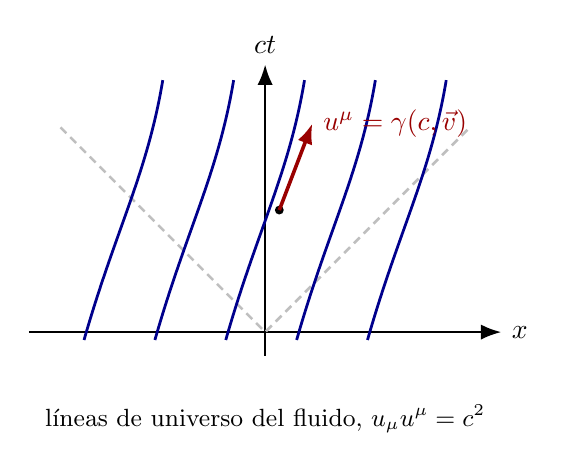
\begin{tikzpicture}[line width=0.9pt,>={Latex[length=2.6mm]}]
  \draw[->] (-3,0)--(3,0) node[right]{$x$};
  \draw[->] (0,-0.3)--(0,3.4) node[above]{$ct$};
  % cono de luz tenue
  \draw[gray!50,densely dashed] (-2.6,2.6)--(0,0)--(2.6,2.6);
  % lineas de universo de elementos fluidos (temporales)
  \foreach \xa in {-1.8,-0.9,0,0.9,1.8}
     \draw[blue!55!black,line width=1pt] (\xa-0.5,-0.1) .. controls (\xa-0.1,1.3) and (\xa+0.3,2.0) .. (\xa+0.5,3.2);
  % cuadrivelocidad tangente
  \coordinate (P) at (0.18,1.55);
  \fill (P) circle(1.6pt);
  \draw[->,red!60!black,line width=1.3pt] (P)--++(0.42,1.1) node[right]{$u^\mu=\gamma(c,\vec v)$};
  \node at (0,-1.1){\small líneas de universo del fluido,\ $u_\mu u^\mu=c^2$};
\end{tikzpicture}
\end{document}
